\documentclass{article}
\usepackage[pdftex]{graphicx}
\usepackage{graphics}
\usepackage{color}

\begin{document}

\author{Sebastian Hahn and Karsten Loesing\\{\tt\{sebastian,karsten\}@torproject.org}}
\title{Privacy-preserving Ways to\\Estimate the Number of Tor Users}
%Counting Users in the Tor Network in a Privacy-Preserving Way
\maketitle

\section{Introduction}

The Tor network allows hundreds of thousands of users every day to stay
anonymous online and enables additional tens of thousands of people in
oppressed countries to circumvent local censorship.
At least, these are the orders of magnitude of Tor usage that we assume
at the time of writing this report.
Estimating the number of users in an anonymity network is a hard
problem.
On the one hand, it's important to learn something about the users of a
network to improve its service.
On the other hand, the users of an anonymity network have a high
demand for privacy, which prohibits collecting sensitive information that
is necessary to obtain exact usage statistics.
In this report we describe our approaches to collect aggregated usage
data and derive user number estimates from them.
% cite WESCR 2010 paper?

We start with our two current approaches to estimate the number of
non-censored daily users.
These approaches are based on counting the number of directory
requests that clients make to update their network information.
Clients need to download initial network information from a small fixed
set of relays, the directory authorities, and refresh their network
information in regular intervals from a larger changing set of relays, the
directory mirrors.
We describe our current approach to estimate the number of new and
returning users from requests seen at directory authorities in
Section~\ref{sec:auths} and our estimate of recurring users based on
requests to directory mirrors in Section~\ref{sec:current}.
%from one of a few hundred relays that are configured as directory mirrors.
%We count these requests on a fast directory mirror, which also reports
%what share of the total requests in the network it thinks it has answered.
%We project the total number of requests in the network using the
%self-reported share and divide by the number of requests that each client
%makes to estimate the total number of users.

In Section~\ref{sec:combine}, we extend our current approach to count
recurring users by combining reported directory requests from multiple
directory mirrors.
%We estimate the fraction of observed requests from the number of bytes
%that directory mirrors spend on answering directory requests instead of
%relying on self-reported expected shares.
The result is a less volatile user number estimate with fewer outliers and
missing data points.

The previous approaches have in common that they estimate user numbers
based on the number of directory requests.
In Section~\ref{sec:entry} we discuss an estimation based on the number of
unique IP addresses seen on a fast directory mirror.
Clients open numerous connections to directory mirrors to download
updated network status information such as new consensuses and
the relay descriptors therein.
%There are roughly 2000 relays in the Tor network at the time of writing.
%Clients need to download the descriptors of all relays, so that they can,
%in theory, use any relay for building a circuit.
A quick analysis of the logs of a bootstrapping Tor client reveals that a
relay that is chosen for 5~\% of all directory requests sees at least
two-thirds of all client IP addresses.
% Explain what kind of analysis?
%
%As a result, Tor is going to introduce the concept of \emph{directory
%guards} which makes client select a fixed set of directory mirrors for all
%requests.
%But until directory guards are implemented, 
We can use the number of
unique IP addresses on a fast directory mirror to estimate the number of
daily users.
The presented approach is based on data coming from a single directory
mirror.
Combining unique IP addresses from multiple directory mirrors needs to be
done very carefully and is left for future work.

We sketch a design to introduce a new counting cell type in
Section~\ref{sec:countingcell}.
Clients would send counting cells once a day to counting authorities or
entry guards.
We discuss the attack potential and possible defenses against adversarial actions.
% TODO is there a better word than 'trick'?  yes.

In Section~\ref{sec:bridges} we describe our current approach to count
censored users.
These users cannot connect to the publicly known relays to download
directory information or establish circuits.
Therefore, censored users have to learn about one or more bridge relays
which behave in a similar manner to normal relays except that they are not listed in
the public directory.
%Clients fetch all their directory information and establish all their
%circuits with a bridge as their first entry point into the Tor network.
Bridges report the number of unique IP addresses they see every day.
Our current approach to count censored users is to simply sum up these
unique IP addresses per day.
We discuss shortcomings and propose improvements to derive a better
estimate for censored Tor users.

We conclude with a comparison of the described approaches, identify the
most promising approaches, recommend possible improvements, and outline
future work in Section~\ref{sec:conclusion}.

\section{Counting requests on directory authorities}
\label{sec:auths}

As of mid 2010, we use two approaches to estimate the number of
non-censored Tor users:
The first approach captures the number of new or returning users, the
second approach counts the recurring users.
This distinction comes from the design of our estimates that are both
based on Tor's directory protocol.

Whenever a client bootstraps or when its network information becomes
stale, the client requests a fresh network status, which is a list of all
currently running relays, from the directories.
New clients which do not have any directory information pick one of
a fixed set of hard-coded directory authorities for their request.
There are currently eight such directory authorities, but the set can be
changed whenever a new version of the Tor software is released.
Returning clients with outdated network information take the same
approach.
Recurring clients with still recent network information choose a directory
mirror for their update request.
The approach for counting new and returning users is described in this
section, the approach for counting recurring users in the next section.

Seven out of eight directory authorities report the number of directory
requests they're answering every day.
When we started estimating new and returning users, only one or two
directory authorities were reporting these data.
That is why we weight the requests seen by a single directory authority
with the expected fraction of requests that the directory authority should
see.
In 2009, clients knew about 7 directory authorities of which on average 6
were running at the same time.
Hence, we made the assumption that the directory authorities reporting
request numbers were picked for every sixth request by new and returning
clients.
Even though an eighth directory authority has been added in 2010, only
clients running a recent development version of Tor use this new directory
authority.
We therefore stick with our original assumption that a directory authority
sees 1 out of 6 requests.
We multiply the reported request number by 6 to obtain an estimate of
daily new or returning users.

\begin{figure}[t]
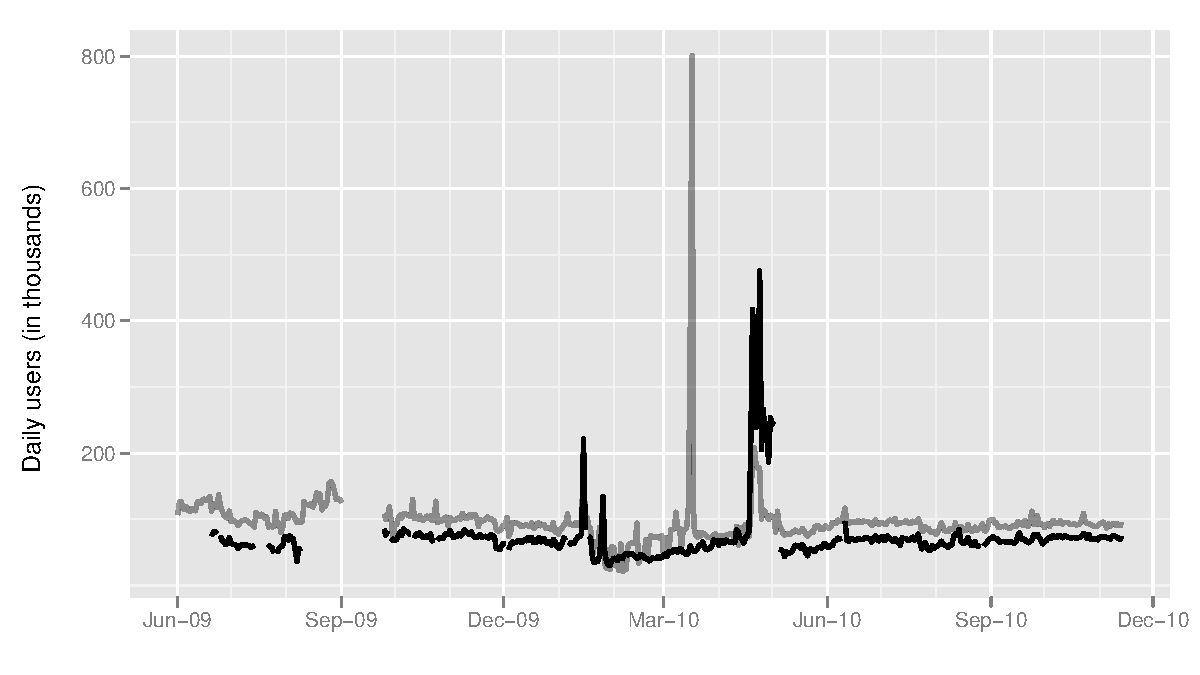
\includegraphics[width=\textwidth]{newusers.pdf}
\caption{Estimated number of new and returning users}
\label{fig:newusers}
\end{figure}

Figure~\ref{fig:newusers} shows the estimated number of new or returning
users based on the request numbers reported by directory authority
\texttt{gabelmoo} (black) and the average reported request numbers by all
directory authorities (gray).
The estimated user number based on the average of all directory
authorities is 20 to 25 thousand users higher than the numbers reported
by \texttt{gabelmoo}, but in general, both estimates are of the same order
of magnitude.
The peak in March 2010 results from a single directory authority reporting
ten times as many requests as the other directory authorities.
This is probably due to a bug in the Tor code and not an actual increase in
users.
The increase in April 2010 can also be explained by bugs in the Tor code
which led to overloading the network.
We therefore expect the average number of new or returning users to be
around 100 thousand.

However, it's difficult to interpret this estimated user number in a
meaningful way.
We don't know how many hours per day a typical user is connected to the
network and after how many hours or days they typically return.
We are more interested in the total number of users connecting to the
network at least once a day.
This question can better be answered by the estimates described below
which attempt to count the number of recurring users.

\section{Counting requests on directory mirrors}
\label{sec:current}

Our current approach for estimating (recurring) daily users is based on
the fact that every client needs to refresh its network information every
few hours in order to make indistinguishable path selection decisions.
Clients weight their choice of a directory mirror by the relays' bandwidth
capacities in order to load-balance requests.
The idea of this approach is to infer the number of users from the number
of directory requests on a fast directory mirror and weight them with the
request share the reporting directory mirrors expects to see.

For our user number estimation, we count the number of network status
requests on a fast directory mirror.
We first estimate how many network status requests there are in the
network by dividing the local request number by the share of requests that
this particular directory mirror thinks it should see.
As an approximation of the request share, the directory mirror reports
the probability of picking itself if it were a client.
In the second step we estimate the number of users by dividing the global
network status request numbers by 10 on the assumption that every client
makes on average 10 requests per day.
10 is probably a too high number, but one that prevents us from
over-counting our users.
% We could derive some statistics from the Torperfs running on moria to
% support our assumption that 10 is too high.

\begin{equation}
U_t = \frac{r_t}{s_t \times 10}
\end{equation}

\begin{center}
\begin{tabular}{p{0.75cm}p{9cm}}
$U_t$ & User number estimate based on directory requests to directory
mirror \texttt{trusted}\\
$r_t$ & Directory requests to directory mirror \texttt{trusted}\\
$s_t$ & Share of directory requests expected at directory mirror
\texttt{trusted}\\
\end{tabular}
\end{center}

\begin{figure}[t]
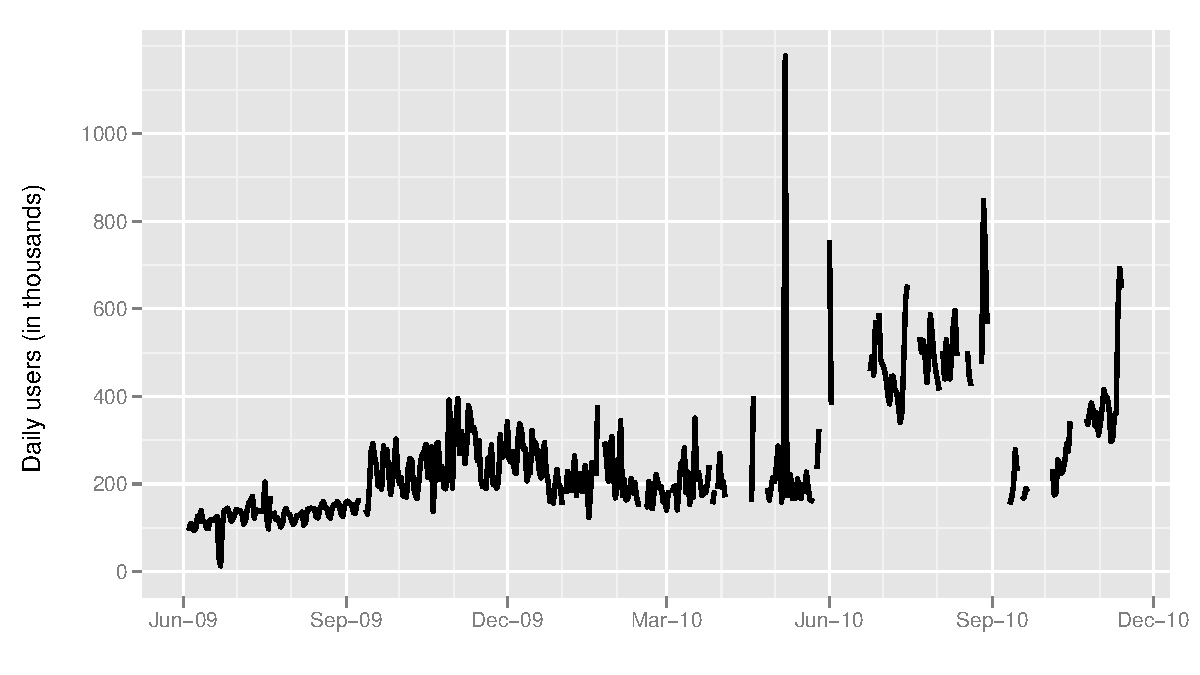
\includegraphics[width=\textwidth]{trusted.pdf}
\caption{User number estimate based on directory requests to directory
mirror \texttt{trusted}}
\label{fig:trusted}
\end{figure}

\begin{figure}[t]
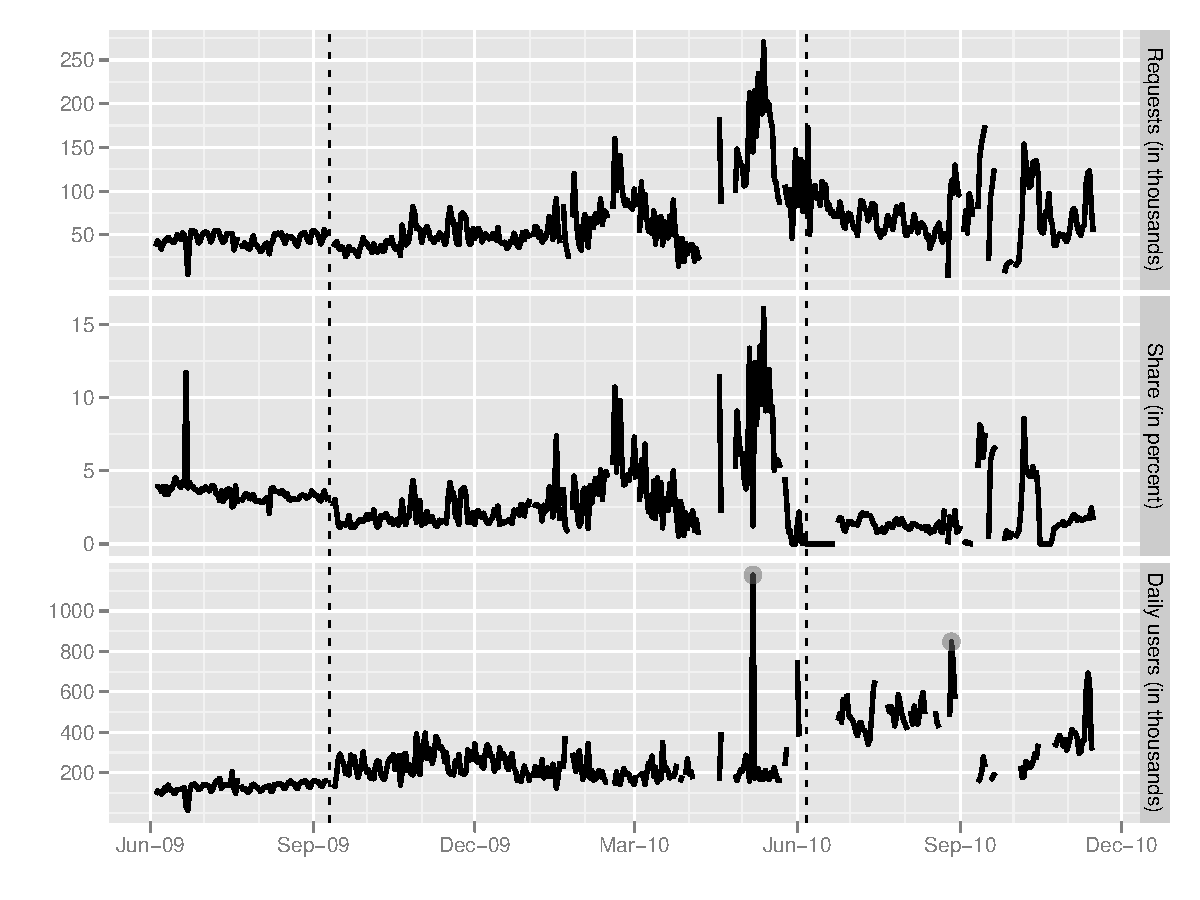
\includegraphics[width=\textwidth]{trusted-details.pdf}
\caption{Directory requests, shares, and user number estimate, based on
directory requests to directory mirror \texttt{trusted}}
\label{fig:trusted-details}
\end{figure}

Figure~\ref{fig:trusted} shows the daily user number estimate based on
directory requests to the fast directory mirror \texttt{trusted}.
Evidently, this estimate is flawed by having outliers and lots of missing
values.
Some of these problems can be explained when looking at the input data.
Figure~\ref{fig:trusted-details} shows the directory requests $r_t$ and
expected share of requests $s_t$ as well as the estimated user number
$U_t$.
From these two graphs we can make a few observations:

\begin{itemize}
\item The peaks in May 2010 and later with 1.2 million and 800
thousand daily users (marked with gray circles) are probably not accurate user
numbers, but more likely measurement errors.
These data points result from directory request shares being slightly
higher than 1~\%.
(Data points with directory request shares of 1~\% or less are excluded
anyway; if these data points were included, there would have been even
more outliers with millions of users which are unlikely real.)
Raising the bar to 1.5~\% would eliminate these outliers, but would also
remove a lot of, apparently correct, data points.
\item In September 2009 (first dashed line), user numbers increased from
roughly 150 to 250 thousand, and volatility of user numbers increased by
factor 2 to 3.
While the request numbers remain more or less stable during this time,
the expected share of requests seen by \texttt{trusted} drops from 3.5~\%
to 2~\%.
The reason for this decrease is that more recent clients started weighting
relays by active bandwidth scanner results instead of the relays'
self-reported bandwidth claims.
However, \texttt{trusted} assumes that all clients use the bandwidth
scanner results for path selection which is not the case.
\item Beginning in June 2010 (second dashed line), shares drop to zero for
about a month, stabilize at around 1.5~\% for two months and then
oscillate between 0 and 9~\%.
The reason for this behavior is the introduction of consensus weights that further help
clients to make good path selection decisions.
Again, \texttt{trusted} bases its expected request share on the
assumption that all clients use consensus weights for their path selection
decisions which is wrong.
\end{itemize}

In summary, the major problem with the described approach is the
approximation of the request share that a directory mirror expects to see.
The various deployed Tor versions all use different weights for picking a
directory mirror:
Clients running Tor version 0.2.0.x use the relays' self-advertised
bandwidths to decide which directory mirror to pick.
Clients on version 0.2.1.x use actively measured bandwidths from four
bandwidth scanners running on the authoritative directory servers for
their choice.
Clients running version 0.2.2.x base their decision on the measured
bandwidths, but weighted by network-wide factors depending on the assigned
relay flags of a directory mirror.
The shares reported by directory mirror \texttt{trusted} reflect a
situation in which all clients run the same Tor version as
\texttt{trusted} at the given time, which is not the case.
While we could calculate shares independent of \texttt{trusted}, we have
no reliable data about the fractions of running client versions and could
therefore not weight the calculated version-specific request shares.
In the next section we discuss an approach to combine the findings of
multiple directory mirrors and replace the expected request share by a
more reliable metric.

% It might also be problematic that relays update their advertised
% bandwidth only every 18 hours when publishing a new descriptor.
% Likewise, bandwidth scanners scan a relay only every so often. There
% may be significant changes from one bandwidth value to the next, but
% clients take a few hours to notice that change. More research would be
% necessary, but we already know the approach is broken, so might as well
% not care.

The second problem with the described approach is that the estimated user
number is less precise the fewer requests a directory mirror sees.
When we started estimating user numbers based on directory mirror
\texttt{trusted}, it reported shares of roughly 3.5~\% of all requests in
the network.
With the introduction of the various performance improvements and with the
recent increase in fast directory mirrors, this share has decreased to
1.5~\%.
As we can see, estimations based on a fraction of observations this small
are not very reliable.

The third problem is that we can only guess that a client makes 10 network
status requests per day.
While this assumption may work for clients which are connected to the Tor
network all day, other clients may well send fewer requests than 10.
We do not have any data about the average hours of Tor usage per day to
come up with a better number than 10 requests.
If, for example, the real number of requests per client was 5, our
estimate would be off by a factor 2.
The good news is that, while being off by an unknown factor, we're off by
that factor all the time, so that comparisons over time are still
accurate.

% Idea for implementing directory guards: With all relays caching
% directory information, instead of building circuits to directories
% *using* directory guards, clients could simply ask their directory
% guards for whatever directory information they want to know.

\section{Combining requests to directory mirrors}
\label{sec:combine}

%\paragraph{Summing up requests and shares}
%
%The first new approach combines directory requests simply by summing up
%requests and shares of all directory mirrors reporting these numbers.
%While \texttt{trusted} was the only fast directory mirror reporting
%directory requests for about a year, a couple of even faster relays
%started reporting these numbers in August 2010.
%
%\begin{equation}
%U_s = \frac{r}{s \times 10}
%\end{equation}
%
%\begin{center}
%\begin{tabular}{p{1cm}p{9cm}}
%$U_s$ & User estimate based on sums of all directory requests and shares\\
%$r$ & Directory requests to all reporting directory mirrors\\
%$s$ & Share of directory requests expected at all reporting directory
%mirrors\\
%\end{tabular}
%\end{center}
%
%\begin{figure}[t]
%\includegraphics[width=\textwidth]{share.png}
%\caption{Directory requests, shares and user number estimate based on
%directory requests by all reporting directory mirrors (black), compared
%to \texttt{trusted} only (gray)}
%\label{fig:share}
%\end{figure}
%
%Figure~\ref{fig:share} shows the total requests, shares, and estimated
%users based on all reporting directory mirrors.
%The total request numbers and reported shares exceed those of
%\texttt{trusted} in May 2010 and from August 2010 on.
%The resulting user number estimate is similar to the current approach
%until May 2010, because \texttt{trusted} was reporting most of the
%requests during that time anyway.
%Beginning in May 2010, the combined numbers have by far fewer missing
%data points, because it's easier to reach shares of 1~\% or higher with
%multiple data source.
%At the same time, the estimated user numbers are lower when combining all
%available data sources.
%
%The results of this new approach are still not satisfactory.
%In particular the estimates of about 1 million users in May 2010 and later
%are hardly correct.
%In addition to that, it's unlikely that the reporting directory mirrors
%saw up to 80~\% of all requests in September and October 2010.
%In the two approaches below we drop the self-reported expected directory
%request shares completely and use different metrics to answer what
%fraction of directory requests have been reported on a given day.
%
%\paragraph{Estimating total requests using bandwidth histories}
%
%The second new approach to combine directory requests makes use of
%bandwidth histories to estimate what fraction of directory requests has
%been reported.
%Rather than resembling clients' decisions for selecting relays (which can
%be difficult with the different deployed path selection strategies), we
%use the bandwidth histories reported by relays to estimate what fraction
%of directory requests they have seen.
%If all directory mirrors reporting directory requests together have
%pushed $b_{pr}$ bytes and all directory mirrors, whether or not they
%report directory requests, have pushed $b_p$ bytes, we expect that in the
%whole network, there have been $\frac{b_p}{b_{pr}}$ as many directory
%requests as we have seen.
%The underlying assumption is that the directory mirrors reporting
%directory requests spend the same fraction of bytes on answering directory
%requests as all directory mirrors.
%
%\begin{equation}
%U_p = r \times \frac{b_p}{b_{pr} \times 10}
%\end{equation}
%
%\begin{center}
%\begin{tabular}{p{1cm}p{9cm}}
%$U_p$ & User estimate based on directory requests to all reporting
%directory mirrors, weighted by bandwidth histories\\
%$r$ & Directory requests answered by all reporting directory mirrors\\
%$b_p$ & Written and read bytes by all directory mirrors\\
%$b_{pr}$ & Written and read bytes by directory mirrors that report
%directory requests\\
%\end{tabular}
%\end{center}
%
%\begin{figure}[t]
%\includegraphics[width=\textwidth]{bwhist.png}
%\caption{Directory requests, shares and user number estimate based on
%directory requests weighted by bandwidth histories}
%\label{fig:bwhist}
%\end{figure}
%
%Figure~\ref{fig:bwhist} shows the estimated users based on directory
%requests weighted by written and read bytes of reporting directory mirrors
%compared to all directory mirrors.
%The user number estimate is less volatile than the previous two estimates
%and has no outliers in the millions.
%There are also only very few missing data points, because the share is
%above 1~\% most of the time.
%
%However, the range of 50 to 500 thousand daily users is still higher than
%expected.
%It might be that the assumption that directory mirrors reporting directory
%requests spend the same fraction of bytes on answering directory requests
%as all directory mirrors is inaccurate.
%We hope that this assumption becomes less important with an even higher
%number of directory mirrors reporting directory requests in the future.

The major shortcomings of the approach described in the previous section
are very low request shares of 1.5~\% or less and the difficulty to
accurately estimate shares of directory requests seen at directory mirrors.
In this section we discuss a new approach to overcome these two problems.
The presented approach combines the reported directory request numbers
from multiple directory mirrors and uses the relays' bandwidth histories
to determine what fraction of the total requests in the network have been
reported.

This new approach utilizes a recently introduced metric: bytes spent on
answering directory requests.
Directory mirrors running Tor version 0.2.2.15-alpha or higher report
how many bytes they spent on answering directory requests in addition to
the number of bytes they spent on all traffic.
By looking at the relay descriptor archives, we can estimate the number of
directory bytes written on a give day by both the relays reporting directory requests and all
directory mirrors (including those that did not report directory requests).

As a first step we estimate the number of directory bytes written by
directory mirrors.
Only a fraction of the directory mirrors are running Tor version
0.2.2.15-alpha or higher, which is why we have to extrapolate the number
of directory bytes from the reported number.
For the first estimation we assume that every directory mirror spends the
same fraction of its total bytes on answering directory requests.
Hence, the reported number of directory bytes constitute a fraction of
total directory bytes in the network that is equal to the number of bytes
written by directory mirrors reporting directory bytes divided by the
number of bytes written by all directory mirrors.
%
%\begin{equation}
%d_p = \frac{d \times b_p}{b_d}
%\end{equation}
%
%\begin{center}
%\begin{tabular}{p{1cm}p{9cm}}
%$d_p$ & Estimated directory bytes\\
%$d$ & Reported directory bytes\\
%$b_p$ & Reported written bytes by all directory mirrors\\
%$b_d$ & Reported written bytes by directory mirrors reporting directory
%bytes\\
%\end{tabular}
%\end{center}

For the second estimation we assume that the difference between total
written and total read bytes on directory mirrors is to a large extent the
result of answering small directory requests with large directory objects.
We observed that relays that don't mirror the directory write more bytes
than they read, too, but the difference between written and read bytes is
much smaller than on directory mirrors.
We weight the bytes written by directory mirrors with the quotient of
read and written bytes on relays that don't mirror the directory in order
to account for non-directory related factors.
We then subtract the number of bytes read by directory mirrors and obtain
an estimate of directory bytes written by directory mirrors.

\begin{figure}[t]
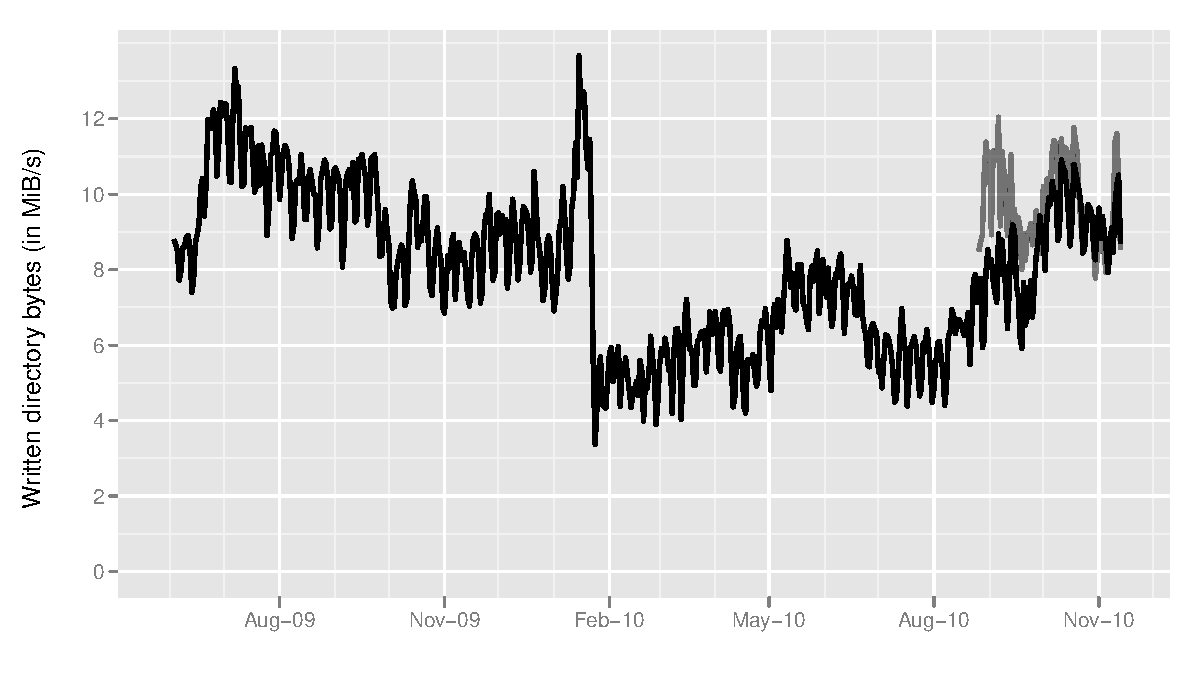
\includegraphics[width=\textwidth]{dirbytes-mirrors.pdf}
\caption{Estimated directory bytes written by directory mirrors based on
the extrapolation of reported directory bytes (gray) and the difference
between written and read bytes (black)}
\label{fig:dirbytes-mirrors}
\end{figure}

Figure~\ref{fig:dirbytes-mirrors} shows the two directory bytes
estimations.
Until mid-September 2010, the extrapolation of reported directory bytes
(gray) is slightly higher than the difference between written and read
bytes (black), but both estimates are of the same order of magnitude.
The difference of up to 4~MiB/s is not much when comparing it to the total
number of bytes written by directory mirrors, which is 300~MiB/s at the
time of writing.
With only three months of data, it is unclear which of the two estimates
is more accurate.
For the following analysis we use the difference between written and read
bytes as estimate for directory bytes, because these numbers are available
for the past 1.5 years.
Once we have a larger fraction of directory mirrors reporting directory
bytes we are going to revisit and possibly adjust this estimate.

Now that we have an estimate of directory bytes written by all directory
mirrors and by the directory mirrors reporting directory requests, we can
extrapolate the number of observed directory requests to learn the total
number of directory requests in the network.
We assume that directory mirrors reporting directory requests spend the
same fraction of directory bytes on answering directory requests as all
directory mirrors.

\begin{equation}
U_d = \frac{r \times (b^w_p \times \frac{b^r_n}{b^w_n} - b^r_p)}{(b^w_{pr} \times \frac{b^r_n}{b^w_n} - b^r_{pr}) \times 10}
\end{equation}

\begin{center}
\begin{tabular}{p{0.75cm}p{9cm}}
$U_d$ & User number estimate based on multiple directory mirrors reporting
directory requests\\
$r$ & Reported directory requests\\
$b^w_p$ & Total bytes written by all directory mirrors\\
$b^r_p$ & Total bytes read by all directory mirrors\\
$b^w_n$ & Total bytes written by all relays that don't mirror the
directory\\
$b^r_n$ & Total bytes read by all relays that don't mirror the directory\\
$b^w_{pr}$ & Total bytes written by all directory mirrors reporting
directory requests\\
$b^r_{pr}$ & Total bytes read by all directory mirrors reporting directory
requests\\
\end{tabular}
\end{center}

\begin{figure}[t]
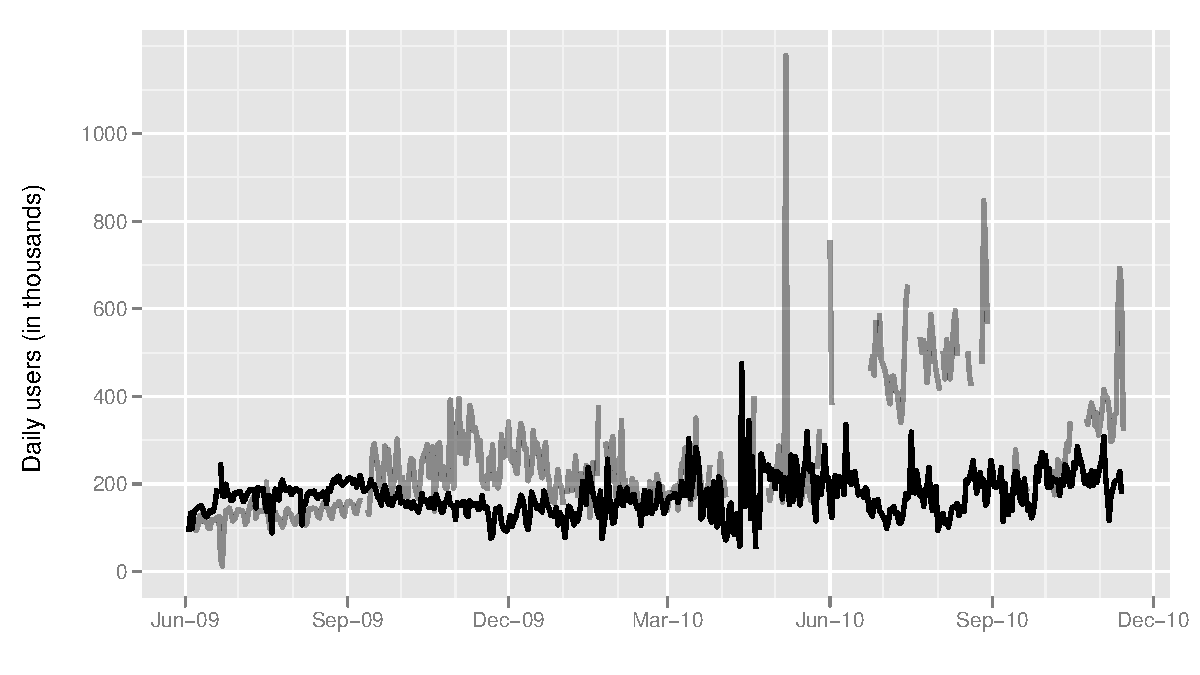
\includegraphics[width=\textwidth]{estimated-users.pdf}
\caption{User number estimate based on all reported directory requests
weighted by estimated written directory bytes (black) compared to the
current approach based on directory requests to directory mirror
\texttt{trusted} (gray)}
\label{fig:estimated-users}
\end{figure}

Figure~\ref{fig:estimated-users} shows the new user number estimate
(black) and compares it to the current approach (gray).
The new user number estimate is less volatile and has no outliers in the
millions.
There are also no missing data points anymore, because the combined
directory requests originate from a fraction of directory mirrors that is
greater than 1~\% in the observed time interval.

%We recommend to increase the fraction of directory mirrors reporting
%directory requests to have a more solid data basis.
%Possible next steps are to ask relay operators running fast and stable
%relays to collect and report these aggregate statistics.
%Further, the configuration option for reporting directory requests could
%be set by default for all relays.
%Once we have more data, we are going to revisit this approach and maybe
%fine-tune it.

%\paragraph{Projecting requests using read/written directory bytes}
%
%We need to learn two data points to calculate what fraction of directory
%bytes the directory mirrors reporting directory requests have pushed.
%First, we need to calculate the number of directory bytes that all
%directory mirrors in the network pushed.
%
%\begin{verbatim}
%We need to find out what fraction of dirreqs are reported to us.
%We assume that the number of dirreqs that a relay answers scales
%proportionally to the number of dirbytes that the relay pushes, i.e., a
%relay that pushes 10 % of all dirbytes also answers 10 % of all dirreqs.
%We need to learn two things in order to answer this question:
%First, how many dirbytes did all relays in the network push?
%Second, how many dirbytes did the relays that report dirreqs push?
%
%We'll start by answering the first subproblem.
%We'd like to learn how many dirbytes were read/written in the network,
%but not all relays report dirbytes.
%Therefore, we weight the reported dirbytes with the fraction of total
%(non-dir) bytes that the relays reporting dirbytes pushed as compared to
%all pushed bytes.
%In order to answer the first question, we count:
%
%b: total reported bytes
%d: total reported dirbytes
%b_d: bytes reported by relays reporting dirbytes
%
%We then can estimate the total number of dirbytes.
%
%D = d * b / b_d
%D: total estimated dirbytes
%
%<dirbytes-total.png>
%
%We need to make sure that enough relays report dirbytes, or our
%extrapolation is based on too few data points.
%The fraction of bytes reported by relays that report dirbytes shouldn't
%
%drop below, say, 15 %.
%The graph only shows data for the fraction being 15 % or higher.
%
%f_bd = b_d / b
%f_bd: fraction of bytes reported by relays that report dirbytes
%
%The second sub problem to solve is to find out how many dirbytes have been
%pushed by the relays that report dirreqs.
%We again use the non-dir bytes that are reported by all relays for the
%extrapolation.
%We count:
%
%d_r:  dirbytes reported by relays reporting dirreqs
%b_r:  bytes reported by relays reporting dirreqs
%b_dr: bytes reported by relays reporting dirbytes and dirreqs
%
%We can then estimate the number of dirbytes being pushed by all relays
%reporting dirreqs.
%
%D_r = d_r * b_r / b_dr
%D_r: total estimated dirbytes reported by relays reporting dirreqs
%
%<dirbytes-part.png>
%
%Finally, we can estimate the total number of dirreqs by using the two
%estimates calculated above.
%
%R = r * D / D_r = r * (d * b / b_d) / (d_r * b_r / b_dr)
%R: total estimated dirreqs, different approaches
%
%Finally assume that each user makes 10 requests per day:
%U = R / 10
%U: total estimate daily users
%
%\end{verbatim}

\section{Counting IP addresses at directory mirrors}
\label{sec:entry}

An alternative approach to count daily users is to count unique IP
addresses on a relay that sees most of the clients at least once a day.
A fast directory mirror is such a relay.
Clients open numerous connections to directory mirrors, in addition to
downloading network statuses, to download relay descriptors.
The Tor network consists of roughly 2000 relays at the time of writing,
and clients attempt to download all relay descriptors, so that they can
build circuits with any of these relays.
Clients split downloads among directory mirrors, because requests cannot
contain more than 96 relay descriptor identifiers.

A quick analysis shows that an always running Tor client sends out on
average 80 requests for relay descriptors per day.
The probability of a fast directory mirror, say, one that is chosen for
5~\% of all directory requests, to be contacted at least once a day is
$1-0.95^{80} = 98.3\%$.
Even a client that only connects to the network for a few minutes per day
downloads all current descriptors which takes at least
$\lceil2000 / 96\rceil = 21$ requests.
The probability of such a client contacting a directory mirror that sees
5~\% of all requests is $1-0.95^{21} = 65.9\%$.

In the near future, Tor is going to introduce \emph{directory guards}.
The idea is that clients pick a small number of relays as their directory
guards and send all directory requests to them.
This is meant to prevent a single malicious directory mirror from learning
about many client IP addresses.
But until directory guards are implemented, we can use the number of
unique IP addresses observed on a fast directory mirror to estimate the
number of daily users.

\begin{figure}[t]
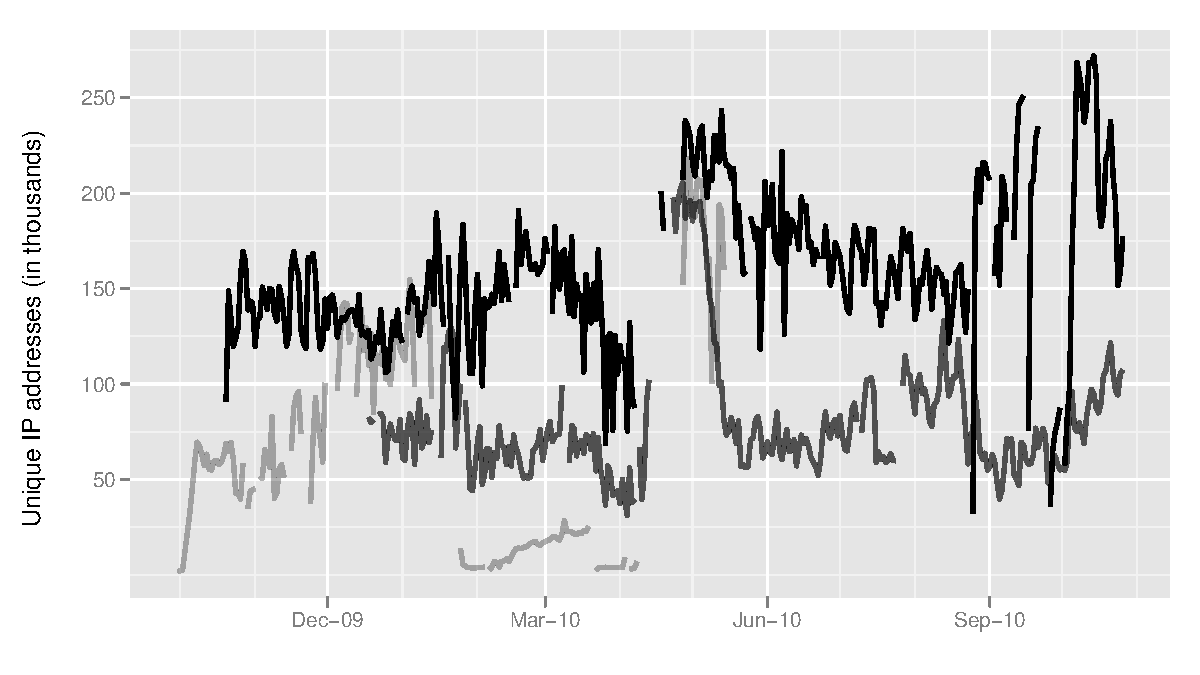
\includegraphics[width=\textwidth]{entrystats.pdf}
\caption{User number estimates based on unique IP addresses reported by
the fast directory mirror \texttt{trusted} (black) and two other fast
directory mirrors}
\label{fig:entrystats}
\end{figure}

Figure~\ref{fig:entrystats} shows the user number estimates
based on unique IP addresses seen on three fast directory mirrors.
The fast directory mirror {\tt trusted} reports the highest number of
unique IP addresses of all three directory mirrors.
There are two time intervals when two or all three directory mirrors
report similar numbers: from December 2009 to January 2010 and from late
April to early May 2010.
The fact that the directory mirrors report similar numbers during those
times is an indication that they all saw the majority of clients in the
network.
We therefore believe that the user number estimates of 150 to 250 thousand
daily users are accurate and pose a realistic upper bound of the real
number of daily Tor users.
These estimates are also of the same order of magnitude as the estimates
described in the previous section.

The major shortcoming of the described approach is that there is no simple
way to combine reported unique IP addresses of two or more directory
mirrors.
Directory mirrors keep the observed client IP addresses in memory for at
most 24 hours, report the absolute number of distinct addresses, and
discard the IP addresses.
It may be possible to exchange data structures containing IP addresses
between directory mirrors in a privacy-preserving way and combine them to
learn about the union size of unique IP address sets.
Possible approaches might be based on private set intersection techniques
or probabilistic data structures like Bloom filters.
We leave these approaches as future work.

\section{Introducing a counting cell}
\label{sec:countingcell}

Another approach is to introduce a new cell type to the Tor protocol; the counting cell.
This approach doesn't estimate user numbers by counting directory
requests or unique IP addresses.
Under this approach, clients would send counting cells once per day to special relays, called
counting authorities.

\subsection{Counting cell overview}
The most important statistic for Tor's user count is the number of daily
users.
Our other metrics are passive observations by certain routers,
whereas the counting cell would be an active approach.
Tor clients would send a notification of their presence once daily, so that
the presence notifications can be added together to get the user count.
Tor has a notion of different cell types to encapsulate different information
when sending it along a circuit.
A new type of cell can easily be created to transport presence information.
This presence information is then reported to the metrics engine and
aggregated to find the actual user count for one day.

Two different approaches are examined here:
The first approach uses Tor's directory authorities as counting authorities.
Clients report their presence via an anonymized tunnel.
Picking guard nodes as counting authorities is the other possibility.
Clients would not need to create a special circuit and can instead just use
one of their regular circuits to send the counting cell to the first hop directly.

Some general considerations are valid for both types:
Counting authorities have to be very stable and well-connected so that
clients can report their presence reliably.
The counting authorities also need to export the data they received in
some document that can be collected by the metrics engine to analyze and
present the statistics.
Tor already has an extra-info descriptor mechanism in place that can be
used.

\subsection{Using directory authorities as counting authorities}
Directory authorities have the same requirements as outlined above:
They need to be very stable, because everyone relies on them to
generate and sign the consensus.
They also already export their votes which get collected by the metrics
engine.

Two options are available for how clients report their presence to these
counting authorities; they can either send a counting cell to each of
them or pick one at random.
Both approaches have advantages and drawbacks, outlined below:

Sending the cell to all authorities might raise a scalability
problem as a single counting authority might not be able to keep
up with the load if all clients make one connection per day to report
their presence.
In a network with 250,000 users, an average of almost 3 reports per
second is to be expected.
In reality, since Tor's user base isn't distributed among timezones
equally, much higher report rates per second are to be anticipated.
The load this induces on each directory authorities should be carefully
examined, because it will increase proportional to an increase in the
user base.

The advantage of reporting presence to all counting authorities is that
if a single report fails, the others can still count the user.
If any of the counting authorities reports a much lower value than
the others for a specific day, it can be taken out of the statistics
aggregating process for that day or until the connectivity problems
are resolved.

Sending a counting cell to just one counting authority increases the
scalability of the system, as new counting authorities
could easily be added once the others are becoming overloaded.
Another advantage is that the user doesn't have to create one circuit
per counting authority, but rather just one per day.
This means that a user who doesn't use Tor for very long on a certain
day can still be counted correctly, even if she wouldn't have had the
time to report her presence to all authorities.


Data loss or other malfunctions on one of the counting authorities
poses a major problem in this scheme.
Such data loss cannot be corrected, and statistics for the time period
will be inaccurate.

\paragraph{Abuse potential and inaccuracies}

In a system where cells are reported to all counting authorities,
there is no strong protection against a counting authority that
increases the count of users by reporting a higher number of users by
just sending counting cells to the other authorities.
It would, however, prevent an authority from under-reporting the number
of users, because the others will report a higher user count so that
the data from the dishonest authority can be discarded by the statistics
aggregator.

When users report their presence to only one counting authority, this
counting authority can under-report the number of users,
because under-reporting cannot be distinguished from being unavailable
for a part of the day.
It is also possible to increase the count of users even without sending
counting cells to the other counting authorities.
Detection of such behavior is very difficult, as lower numbers can
always be explained to be due to network problems at the counting
authority; and only very unusually high numbers would indicate increasing
the number of users maliciously.

It is trivial to arbitrarily increase the count of users by sending on
average more than one counting cell per 24 hour window.
Because counting cells are anonymized, there are no special resources
necessary to execute the attack, other than the ability to make circuits
to the counting authorities.
This attack needs to be continued for as long as the user count is to be
influenced.
When the attack is stopped, the result will be an apparent loss of Tor
users.

When the scheme is newly deployed or when alternative
implementations of Tor clients that don't include counting cells are
introduced, the number of Tor users will be undercounted.
Both cases have to be taken into consideration when evaluating the
collected data.

\paragraph{Possibility for additional statistics}
Because clients report their presence anonymously under the counting cell scheme, additional statistics
can be gathered using this approach.

Example statistics are client version and the uptime since the last
cell was sent.
%
While adding additional statistics, care must be taken that the anonymity
set is still sufficiently large.
For the client version, we could report the accurate version while it is
still recommended or ``outdated'' as a catch-all for older versions.
%
For the uptime since the last cell was sent, reporting uptime in half-hour
time intervals could provide proficient accuracy.

More work is necessary to evaluate the additional risks of adding more
statistics.
If these statistics are deemed important, they can
use the same infrastructure set up for user number estimation.
Directory authorities are expected to be upgraded quickly, so the
new statistics would become available as soon as enough clients
upgrade.


\subsection{Using entry guards as counting authorities}
To address the scalability concerns outlined above, an alternative approach
is to use the entry guards that a client connects to anyway.
Not reporting presence information via an anonymized channel to one
of the chosen guard nodes has the advantage of being more scalable
than either proposed system.
The entry guards can keep track of which IP addresses have already
reported presence information on a given day and refuse
to accept another counting cell.
Also, availability concerns are reduced because a given entry guard
will see fewer counting cells compared to a counting authority.

Guards that support acting as counting authorities and choose to do so
should be marked as such in the consensus by a special flag
so that clients can see which relays are acting as counting authorities.

\paragraph{Abuse potential and inaccuracies}
Using entry guards as counting authorities gives them the same
abuse abilities as directory authorities have in the system where
presence information is reported to one of them; but it could be easier
to filter out extreme values as the reported values are expected to
be generally lower.

The directory authorities should make sure that enough guards exist
so that over and undercounting guards can be detected and excluded
by the metrics engine.

\paragraph{Possibility for additional statistics}
Because guards know who is connecting to them, there is more concern
when adding additional statistics compared to the directory authority
approach.
By including additional information about their presence, Tor clients add
bits of information that can help identify them across IP address changes.
This must be prevented, so additional statistics can not be implemented
when using guard nodes without further analysis showing their safety.

\subsection{Usefulness of counting cells}
Because of the presented attacks, counting cells are likely to be useful
in addition to other user number estimation schemes only.
They can, however, provide an easy way to evaluate trends and
might allow new statistics to be gathered.

\section{Counting IP addresses at bridges}
\label{sec:bridges}

As a special case of counting Tor users, we are interested in the number
of censored Tor users connecting via bridges.
Censored users cannot connect to the publicly known relays to download
directory information or establish circuits.
Censored users have to learn about one or more bridge relays which are
similar to normal relays except that they are not listed in the public
directory and are therefore harder to block.
Bridge clients fetch all their directory information and establish all
their circuits with a bridge as first entry point into the Tor network.
Bridges report the number of unique IP addresses they see every day.
Our current approach to count censored users is to simply sum up these
unique IP addresses per day and interpret the result as estimated user
number.

\begin{figure}
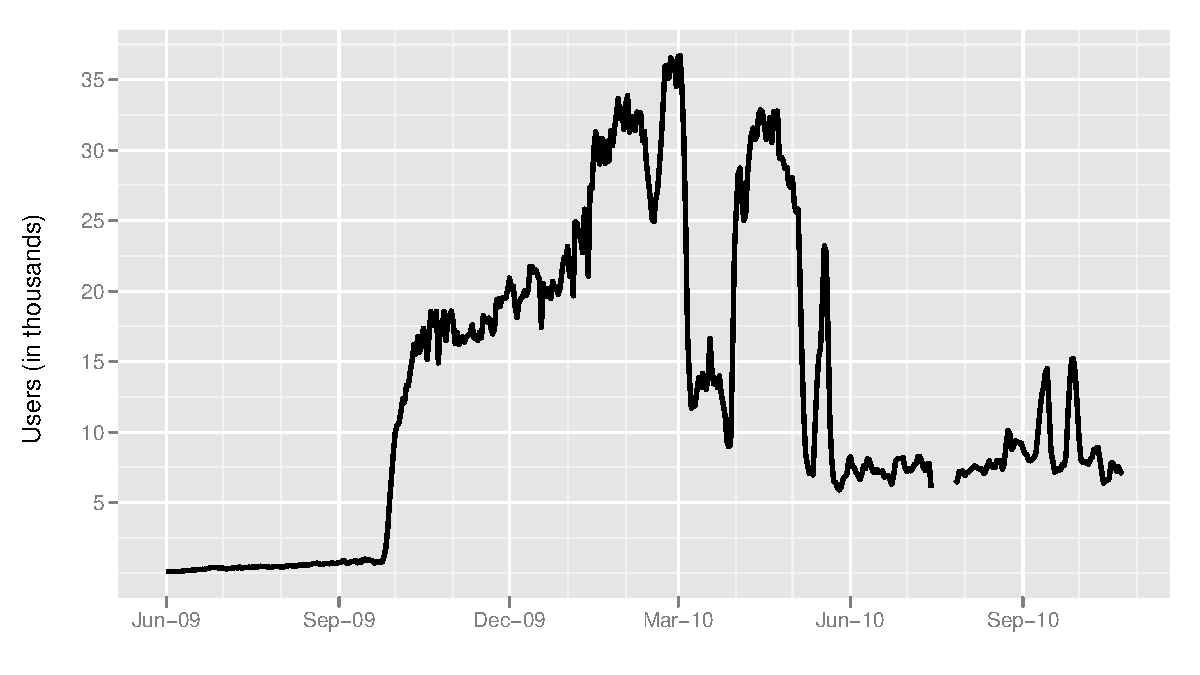
\includegraphics[width=\textwidth]{bridge-users.pdf}
\caption{Estimated number of users connecting via bridges}
\label{fig:bridge-users}
\end{figure}

Figure~\ref{fig:bridge-users} shows the estimated number of users
connecting via bridges.
These numbers are not expected to be as stable as the number of directly
connecting users, because some countries have successfully blocked relays or
even bridges in the past, which has led to sudden increases or decreases in
bridge user numbers.

There are some shortcomings with this approach to count bridge users.
First, the approach makes the assumption that bridge users only connect to
a single bridge every day which is not necessarily the case.
As a result we may over-count bridge clients connecting to two or more
bridges.

The second shortcoming is that we're excluding between 15 and 50~\% of
bridges from the statistics for various reasons:
bridges with fewer than 24 hours uptime are excluded, because bridges only
report statistics every 24 hours to hide the exact connection times and
protect the bridge users' privacy;
bridges that have been running as a non-bridge relay are excluded, because
they might report non-bridge users;
bridges without a GeoIP database are excluded, because they don't report
any statistics about connecting clients;
bridges running a few early versions of the 0.2.2 series are excluded,
because they had a bug in reporting bridge user statistics;
finally, an unknown number of bridges is excluded, because bridge
operators decide not to publish their bridge to the bridge authority and
circulate the bridge address to bridge users themselves.

In the future, we might count the number of directory requests to bridges
in the same way as we do on directory mirrors.
Bridge clients need to refresh their view of the network at regular
intervals, too.
So, it should be possible to count bridge users in the same way as we
estimate directly connecting users.

\section{Conclusion}
\label{sec:conclusion}

In this report we described our current approaches to estimate daily Tor
users based on counting directory requests and unique IP addresses, and we
sketched a design to introduce special counting cells for this purpose.
We conclude with a brief summary.

In Section~\ref{sec:auths} we discussed our current approaches for
counting new and returning as well as recurring users based on counting
directory requests.
We found that it is hard to interpret the estimate of new and returning
users without knowing how many hours per day our users are connected and
after how many hours or days they return.
We suggest discontinuance of this statistic because the rather
technical distinction between new/returning and recurring users is not
obvious.

We described our approach to estimate recurring users based on directory
requests reported by directory mirror \texttt{trusted} in
Section~\ref{sec:current}.
We are facing two major problems with this approach, namely approximating
the request share that \texttt{trusted} can expect to see and the decrease
of said share over the past 12 months.
We recommend discontinuance of this statistic as well and recommend replacing it with a
statistic based on directory requests reported by multiple directory
mirrors.

In Section~\ref{sec:combine} we described such an approach to combine the
directory requests from multiple directory mirrors.
This approach is based on the estimated number of directory bytes written
by directory mirrors.
We hope to gather more data from directory mirrors to improve this
promising approach.
Once we have confirmed its correctness, we propose to replace the current
two approaches to estimate direct users with this approach.

We presented results from counting unique IP addresses on fast directory
mirrors in Section~\ref{sec:entry}.
These results are interesting, because they allow us to determine an upper
bound of daily users.
However, we did not find a simple way to combine reported unique IP
addresses of two or more directory mirrors in a privacy-preserving way.
Once the directory guard design is implemented, this approach won't
deliver useful estimates anymore.
We leave this problem as future work.

In Section~\ref{sec:countingcell} we sketched a new design to introduce
counting cells that clients would send once a day to counting authorities
or entry guards.
Such an approach would allow us to gather better statistics about clients.
However, more work is needed to reduce the potential for abuse.

Finally, in Section~\ref{sec:bridges} we described our current approach to
count censored users.
This statistic is based on the sum of unique IP addresses observed on
bridges with at least 24 hours uptime.
We suggest extending the statistics on bridges to count directory
requests.
We could then try to estimate the number of censored users by weighting
the observations with the bridges' reported bandwidth.
Again, we leave this extension as future work.

\end{document}

